%======================================================================
%===  dtuposter - a class to make posters tha comply with the DTU CI
%
% Written and maintained in 2011-2014 
% by Jorrit Wronski (jowr@mek.dtu.dk)
%
%
%==========================================
%===  details and poster setup
\documentclass[
%    ,title     = {{Title test}}
%    author    = {{Soeren Winkel Holm}}
%    ,subject   = {{This is the subject of my work}}
%    ,bgcolor   = dtulightgreen
%    ,highlight = dtuyellow
%    ,toplogo   = {{tex_dtu_aqua_b_uk}}
%    ,botlogo   = {{tex_dtu_bibliotek_b_uk}}
%    ,papersize = {{a0paper}}
%    ,colcount  = {{1column}}
%    ,longtitle
%    ,largecaption
%    ,draft
%    ,nocrop
%    ,english        % language
%    ,fleqn          % equations on the left
]{dtuposter}
%
%
%======================================================================
%===  Continue with packages
\usepackage[T1]{fontenc}        % special characters
%
%\usepackage[ansinew]{inputenc}  % Windows
%\usepackage[applemac]{inputenc} % MacOS
\usepackage[utf8]{inputenc}    % Unicode, Linux

%
% 
%======================================================================
%=== Font definitions, DTU recommends Arial for posters
%\usepackage{cmbright}
%\usepackage{arevmath}
%\usepackage[scaled]{uarial} %Arial clone, set as default sf font - use "ua1" for direct access
%\usepackage{uarial} %Arial clone, set as default sf font - use "ua1" for direct access
%\usepackage[typeface=default,
%            sanstypeface=urwarial,
%            mathtypeface=arevmath
%           ]{typeface}
\renewcommand{\familydefault}{\sfdefault}
\usepackage{enumitem}
\usepackage{mathtools}
\setlist{nosep,leftmargin=*}
%
% 
%======================================================================
%=== Other useful packages
\usepackage{booktabs}

\usepackage{float}
\usepackage[caption = false]{subfig}
%======================================================================
%=== The actual content starts here
\begin{document}
%
%
%======================================================================
%===  Make header for poster (title and authors)
\begin{dtuposterhead} %
\dtuposterauthor{Mads Andersen, Oskar Wiese, Anders Henriksen, Søren Holm, Asger Schultz}
\dtuposteraffil{DTU Compute}
\dtuposteraffil{\texttt{\{s173934, s183917, s183904, s183911, s183912\}@student.dtu.dk}}
\end{dtuposterhead}
%
%
%======================================================================
%===  ... and the rest of the content
\begin{dtupostercontent}
\section{Weeds, Crops and Dirt}
\begin{itemize}
	\item Agriculture can be made more efficient by using automization to classify seperate the crops from the weeds and the dirt.
	\item On this poster, you can expect to learn about the implementation of SegNet for pixelwise crop classification on a drone image. The results of this implementation is also shown as well as how they came to be.
\end{itemize}
 
\section{The Data: Brazilian Sugar Fields}
The data used in this project is one drone image of a field, which is illustrated as the following.
\begin{figure}
\centering
\includegraphics[width=.7\linewidth]{raw-min2}
\caption{Sugarcane field in Brazil, }
\end{figure}


\section{Our SegNet: 1152 Feature Maps}


%%Model af netværket 
%%Encoder-Decoder
%% "Skip connections"" + Adam 

\begin{figure}
	\centering
	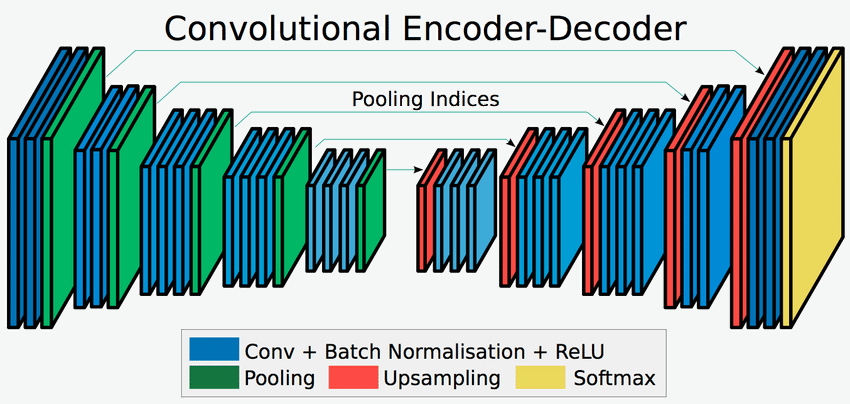
\includegraphics[width=0.9\linewidth]{Encoder-Decoder2}
	\caption{The structure of the network. Dropout prevents overfitting, batchnorm normalizes, ReLU creates non-linearity and max-pool helps with translational invariance.}
	\caption{}
	\label{fig:Structure}
\end{figure}

\begin{itemize}
	\item Same but mirrored encoder and decoder dimensions means ample opportunity for pixel-wise classification!
\end{itemize}
 
%\begin{figure}
%	\centering
%	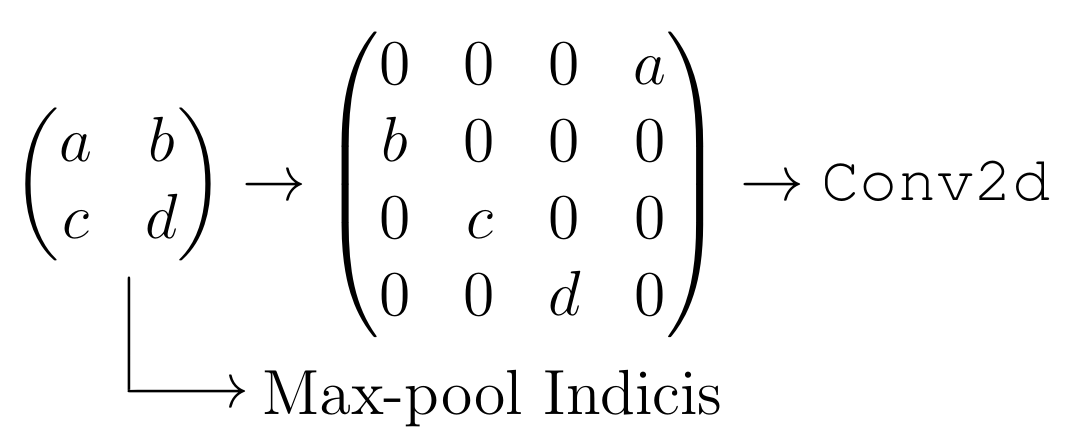
\includegraphics[width=1\linewidth]{pool}
%	\label{fig:maxpool}
%\end{figure}
\subsubsection*{Skip Connections}
The skip connections used in SegNet are the max-pooling indices from the encoder-layer. These indices are used for the up-sampling in the decoder-layers. The process is illustrated as the following:
\begin{equation*}\label{key}
\scriptsize
\begin{bmatrix}a&b\\c&d\end{bmatrix} \xrightarrow{\text{\scriptsize M. pool indices}}
\begin{bmatrix}0&0&0&a\\b&0&0&0\\0&c&0&0\\0&0&d&0\end{bmatrix} 
\rightarrow 
\texttt{\scriptsize Conv2d}
\end{equation*}

Loss of \(N\) pixels in one-hot \((N \times  3)\) matrix \(\mathbf x^\text{pred}\) with the true classes \(\mathbf c\).
\[
L = \underbrace{
\vphantom{\sum_{i}}
\frac 1 N}
_{\mathllap{\text{Mean over minibatch}}}
\sum_{\mathclap {i=1}}^{N}
\underbrace{ 
\vphantom{\sum_{i}}
\mathbf{w}[i, c_i]}
_{\mathclap{\text{Class weight}}}  
\cdot 
\underbrace{
\log 
\frac
{-\exp\mathbf x^\text{pred}[i, c_i]}
{\sum_{j=1}^{3}\exp\mathbf x^\text{pred}[i, j]}
}_{\mathclap{\text{3-class cross entropy}}}
\]
\begin{figure}
	\begin{center}
			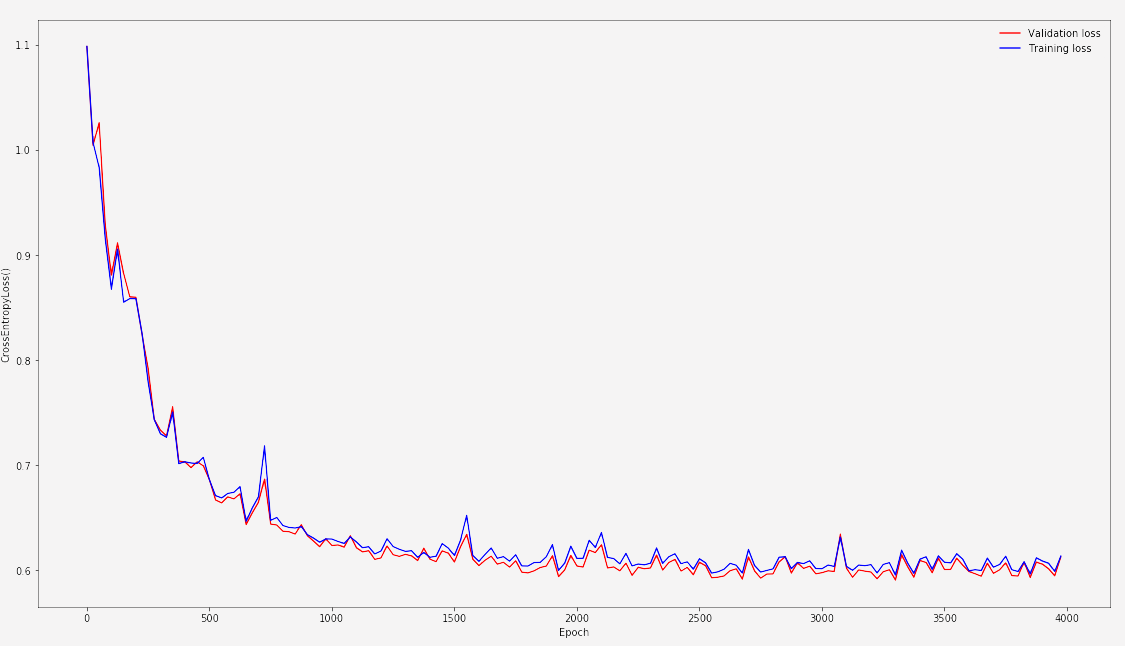
\includegraphics[width=\linewidth,origin=c]{loss2}
	\end{center}
	\caption{An example caption. Figures can be wrapped in the \texttt{fadebox} 
		environment to provide them with a white background. Note that you have to align the 
		figure again.}\label{fig:example2}
\end{figure}

%% Hvordan regulariseres netværket
%% Data transformeringer 
%% Hyperparametre 
\section{Reconstruction}
\begin{figure}
	\centering
	\includegraphics[width=0.7\linewidth]{"Reconstruction DL"}
	\caption{}
	\label{fig:reconstruction-dl}
\end{figure}



\section{Different Metrics, Different Stories}


%%Tabel med metrics 
%% Gøre vores F1 score fed og skriftstørrelse 100
\begin{table}
	\begin{tabular}{c|cccc|cccc|}
		
		\rule[-1ex]{0pt}{2.5ex}  & \multicolumn{4}{c|}{Train} &  \multicolumn{4}{c|}{Test} \\ 
		
		\rule[-1ex]{0pt}{2.5ex} Metric  & G & C &mIoU&  F1 & G & C & mIoU& mF1 \\ 
		\hline
		\rule[-1ex]{0pt}{2.5ex} Baseline&  33.3 &1.8  &3.4  &33.3  &1.1  &2.2  \\ 
		
		\rule[-1ex]{0pt}{2.5ex} USC. SegNet    &  &  &  &  &  &95.9  \\ 
		\rule[-1ex]{0pt}{2.5ex} USC. UNet   &  &  &  &  &  &92.9  \\ 
		\rule[-1ex]{0pt}{2.5ex} Cellari DNN   &  &  &  &  &  &77.7  \\ 
		\hline 
		\rule[-1ex]{0pt}{2.5ex} Our SegNet & 96.5&93.6  & 86.9 &97.5  & 90.7  &\textbf{84.6}  \\ 
	\end{tabular} 
\caption{Conclusions lala note cellari has not provided more scores note U. SC. does not have same test set}
\end{table}



%Kort beskrivelse af resultater 

\begin{figure}
	\centering
\subfloat{
	
\includegraphics[width=.5\linewidth]{target2}	
}
\subfloat{
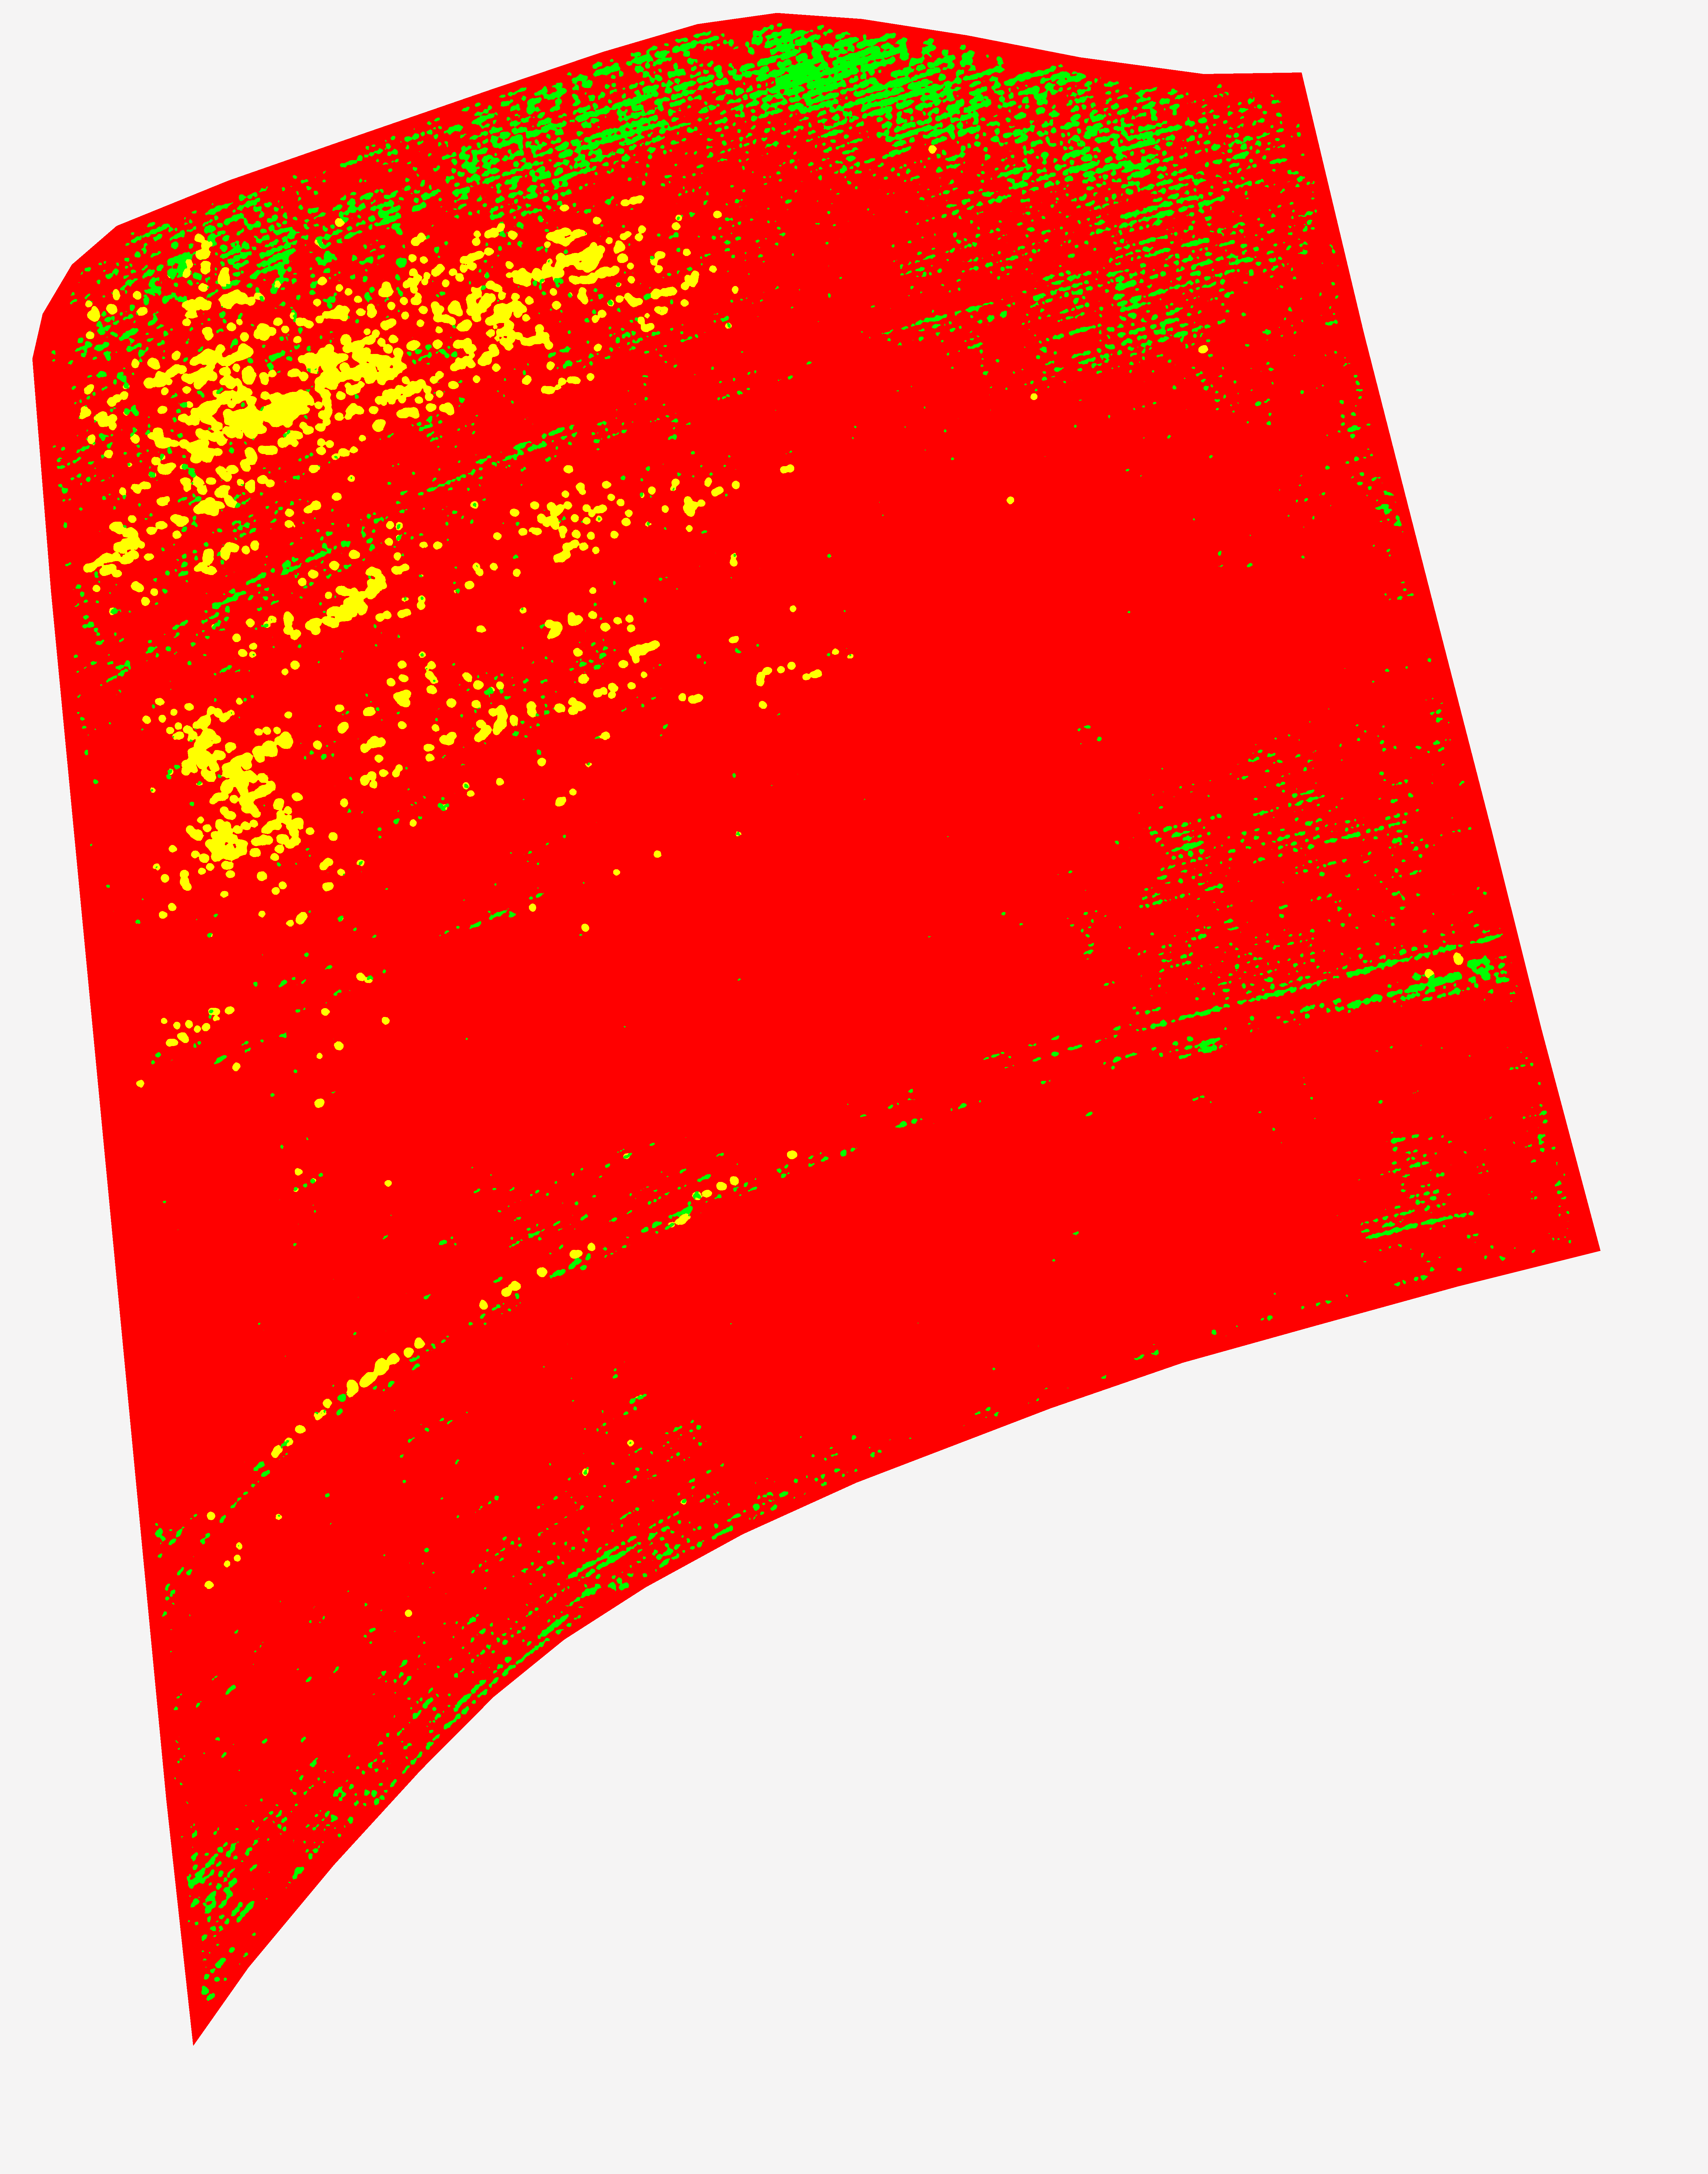
\includegraphics[width=.5\linewidth]{anno}	
}
\caption{An example caption. This figure supports transparency and looks fine on 
the coloured background}\label{fig:example}
\end{figure}



\section{Where Can This Go?}
% Yderligere arbejde
%Perspektiv på problemet 

\begin{figure}
	\begin{center}
			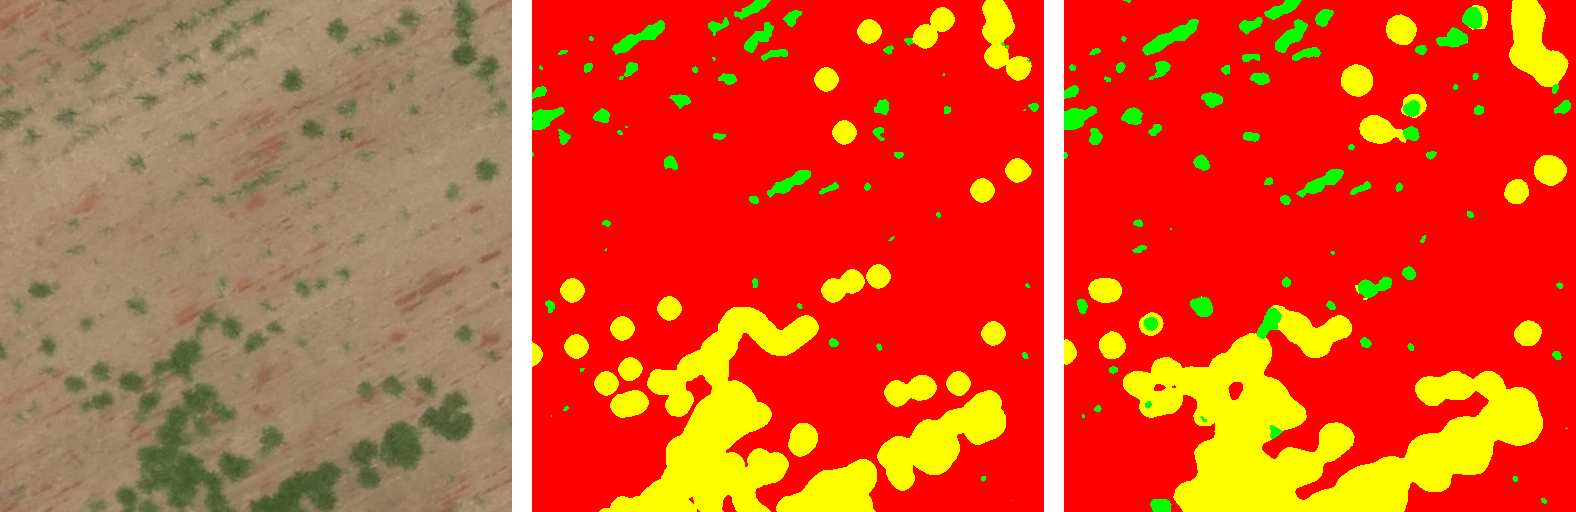
\includegraphics[width=\linewidth,origin=c]{reconst}
	\end{center}
\end{figure}

\begin{itemize}
	\item Complications with the task of image segmentation is the limited amount of data available. 
	\item More data and more advanced data augmentation can lead to a more generalizable and robust model.
	\item Can lead to an algorithm that can indentify crops and weed on a field and aid farmers in their work.
\end{itemize}

\end{dtupostercontent}
\end{document}
